\documentclass[pdf,xcolor=table]{beamer}

\usepackage{default}
%\usepackage[utf8]{inputenc}
\usepackage{subfig}
\usepackage{graphicx}
\usepackage{booktabs}
\graphicspath{{figures/}}
\DeclareGraphicsExtensions{.pdf}
\usepackage{enumitem,amssymb}
\newlist{todolist}{itemize}{2}
\setlist[todolist]{label=$\square$}
\usepackage{pifont}
\newcommand{\cmark}{\ding{51}}%
\newcommand{\xmark}{\ding{55}}%
\newcommand{\done}{\rlap{$\square$}{\raisebox{2pt}{\large\hspace{1pt}\cmark}}%
\hspace{-2.5pt}}
\usepackage{algorithm,algorithmic}
\usepackage{pdfpages}
\usepackage{hyperref}
\usepackage[citestyle=authoryear-comp,
            style=authoryear-comp,
            backend=bibtex]{biblatex}
\bibliography{tese}
\setbeamertemplate{bibliography item}{\insertbiblabel}

\usetheme[sectionpage=progressbar, block=fill]{metropolis}% Use metropolis theme

\title{FCA and an Extension to Graphs}
\subtitle{}
\author[Presenter: Saullo Oliveira - shgo@dca.fee.unicamp.br]{Saullo~H.~G.~de~Oliveira}
\institute{FEEC - University of Campinas - Brazil}
\date{}

\overfullrule=2cm

\begin{document}

\begin{frame}
    \titlepage
\end{frame}

\begin{frame}{Outline}
    \tableofcontents
\end{frame}

\section*{Intro}
\begin{frame}[t]{What is FCA?}
    \begin{itemize}
        \item[$\bullet$] \textit{Formal Concept Analysis} is a field of applied mathematics based on the mathematization of \textit{concept} and \textit{conceptual hierarchy}.
        It thereby activates mathematical thinking for conceptual data analysis and knowledge processing \parencite{Ganter1999}.
        \item[$\bullet$] It tries to formalize our use of concepts and specialization of concepts.
        \item[$\bullet$] FCA is a way of hierarchically represent a relationship between two sets.
    \end{itemize}
\end{frame}

\begin{frame}[t,label=toy]{A Toy Example}
    \begin{columns}
        \begin{column}{0.5\textwidth}
            % Please add the following required packages to your document preamble:
            % \usepackage{booktabs}
            \begin{table}[]
            \tiny
            \centering
            \caption{Toy example}
            \begin{tabular}{@{}|l|l|l|l|@{}}
            \hline
                    & Tem Filhos & Trabalha & Cozinha \\\hline
            Nilson  & X          & X        & X       \\\hline
            Cássia  & X          & X        &         \\\hline
            Aline   & X          & X        &         \\\hline
            Amanda  &            &          & X       \\\hline
            Alan    &            & X        &         \\\hline
            Beatriz &            &          &         \\\hline
            \end{tabular}
            \end{table}
        \end{column}
        \begin{column}{0.5\textwidth}
            \begin{figure}[h]
                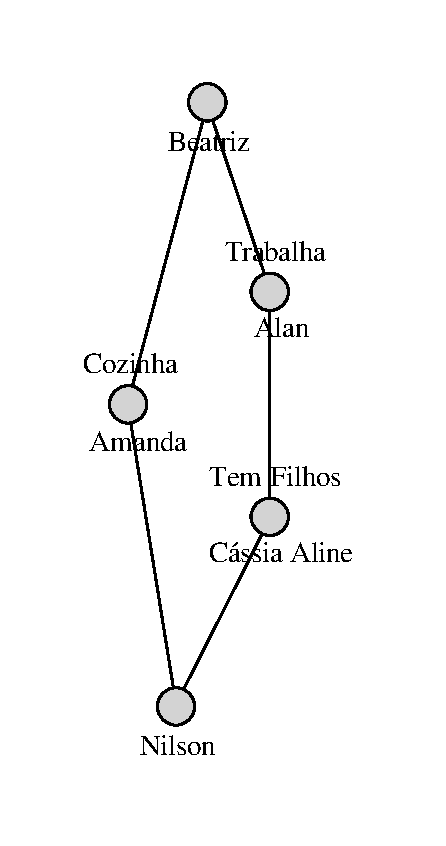
\includegraphics[trim={0pt 2  10 35},clip,height=154pt]{/home/shgo/Dropbox/Doutorado/Palestras/fca/figures/lattice.pdf}
                \caption{Toy example concept lattice.}
            \end{figure}
        \end{column}
    \end{columns}
\end{frame}

\begin{frame}[t]{Checklist for FCA}
    \begin{todolist}
        \item Find a hierarchical order in a set of elements.
        \item Find relationships between two sets.
        \item Find a hierarchical order in a relationship between two sets.
    \end{todolist}
\end{frame}

\section[Ordered Sets and Lattices]{An Introduction to Ordered Sets and Lattices}
\begin{frame}[t]{Binary Relation}
    \begin{definition}[\text{\cite[p. 1]{Ganter1999}}]
    A \textbf{binary relation} \textit{R} between two sets \textit{M} and \textit{N} is a set of pairs $(m, n)$ with $m \in M$ and $n \in N$. Instead of $(m, n) \in R$ we often write $mRn$.
    \end{definition}
    \begin{definition}[\text{\cite[p. 1]{Ganter1999}}]
        A binary relation $R$ on a set $M$ is called an \textbf{order relation}, if for all $x, y, z \in M$:
        \begin{enumerate}
            \item[$\bullet$] Reflexivity: $xRx$
            \item[$\bullet$] Antisymmetry: $xRy$ and $x \ne y \implies$ not $yRx$
            \item[$\bullet$] Transitivity: $xRy$ and $yRz \implies xRz$
        \end{enumerate}
    \end{definition}
\end{frame}

\begin{frame}[t]{Ordered Sets}
    \begin{definition}[\text{\cite[p. 1]{Ganter1999}}]
        An \textbf{ordered set} is a pair $(M, \leq)$, with $M$ being a set and $\leq$ an order relation on $M$.
    \end{definition}
    Examples:
    \begin{itemize}
        \item[$\bullet$] $\mathbb{R}$ with the usual $\leq$ relation.
        \item[$\bullet$] the power set $\mathfrak{B}(X)$ of any set $X$ with set inclusion ($\subseteq$) relation.
    \end{itemize}
\end{frame}

\begin{frame}[t]{Neighbors}
    \begin{definition}[\text{\cite[p. 2]{Ganter1999}}]
        $a$ is a \textbf{lower neighbor} of $b$, if $a < b$ and there is no $c$, such that $a < c < b$. In that case, we write $a \prec b$.
    \end{definition}
    \begin{itemize}
        \item[$\bullet$] $1 \prec 2$ in $(\mathbb{N}, \leq)$
        \item[$\bullet$] $\{0, 1\} \prec \{0, 1, 2\}$ in $(\mathfrak{B}(\{0, 1, 2, 3\}), \subseteq)$
    \end{itemize}
\end{frame}

\begin{frame}[t]{Infimum and Supremum}
    \begin{definition}[\text{\cite[p. 5]{Ganter1999}}]
        Let $(M, \leq)$ be an ordered set and $A \subset M$. A \textbf{lower bound} (\textbf{upper bound}) of $A$ is an element $s \in M$ such that $s \leq a (s \geq a), \forall a \in A$.
    \end{definition}
    \begin{definition}[\text{\cite[p. 5]{Ganter1999}}]
        If there is a largest element in the set of all lower bounds of A, it is called the \textbf{infimum} of A, denoted by $inf\ A$ or $\bigwedge A$. Dually, a least upper bound is called \textbf{supremum}, denoted by $sup\ A$ or $\bigvee A$.
    \end{definition}
\end{frame}

\begin{frame}[t]{Complete Lattices}
    \begin{definition}[\text{\cite[p. 5]{Ganter1999}}]
        An ordered set $\textbf{V} := (V, \leq)$ is a \textbf{lattice}, if for any two elements $x$ and $y$ in $V$, $x \wedge y$ and $x \vee y$ always exist.
        \textbf{V} is called a \textbf{complete lattice}, if $\bigwedge V$ and $\bigvee V$ exist for any subset $X$ of $V$.
    \end{definition}
    \begin{figure}
        \centering
        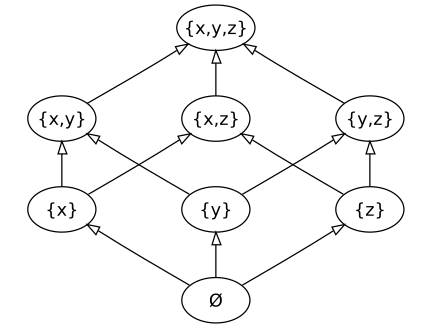
\includegraphics[width=130pt]{Hasse_diagram_of_powerset_of_3.png}
        \caption{Powerset Lattice of the set $\{x, y, z\}$, ordered by inclusion \parencite{lattice}.}
    \end{figure}
\end{frame}

\begin{frame}[t]{Checklist for FCA}
    \begin{todolist}
        \item[\done] Find structure in a set of elements
        \item Find relationships between two sets
        \item Find a structure in a relationship between two sets
    \end{todolist}
\end{frame}

\begin{frame}[t]{Maps Between Posets}
    \begin{definition}[\text{\cite[p. 6]{Smith2010}}]
         Suppose that $\textbf{P} = (P, \leq)$ and $\textbf{Q} = (Q, \leq)$ are two posets. Let $f: P \rightarrow Q$ be a map between the two sets. Then,
        \begin{enumerate}
            \item[(i)]$f$ is monotone \textit{iff}, for all $p, p' \in P$, if $p \leq p'$ then $f(p) \leq f(p')$
            \item[(ii)] $f$ is order-embedding \textit{iff} for all $p, p' \in P$, $p \leq p'$ iff $f(p) \leq f(p')$
        \end{enumerate}
    \end{definition}
    Important observations
    \begin{itemize}
        \item[$\bullet$] A map can squeeze all elements.
        \item[$\bullet$] $f$ is an injective (one-one) map.
        \item[$\bullet$] if $f$ is an order-embedding map, and is an onto function, $f$ is an order-isomorphism.
    \end{itemize}
\end{frame}

\begin{frame}[t]{A special case: Galois Connection}
    \begin{definition}[\text{\cite[p. 12]{Smith2010}}]
        Let $\textbf{P} = (P, \leq)$ and $\textbf{Q} = (Q, \leq)$ be posets.
        Suppose $f^{\uparrow}: P \rightarrow Q$ and $f^{\downarrow}: Q \rightarrow P$ are a pair of functions such that for all $p \in P, q \in Q:$
            \begin{equation}
                f^{\uparrow}(p) \leq q \iff p \leq f^{\downarrow}(q).
            \end{equation}
        Then the pair $(f^\uparrow, f^\downarrow)$ form a Galois connection between $\textbf{P}$ and $\textbf{Q}$.
    \end{definition}
\end{frame}

\begin{frame}[t]{Galois Connection}
    \begin{theorem}[Alternative definition, \text{\cite[p. 15]{Smith2010}}]
        Let $\textbf{P} = (P, \leq)$ and $\textbf{Q} = (Q, \leq)$ be posets.
        Suppose $f^{\uparrow}: P \rightarrow Q$ and $f^{\downarrow}: Q \rightarrow P$ are a pair of functions between the two sets. Then $(f^\uparrow, f^\downarrow)$ is a Galois connection if and only if:
        \begin{itemize}
            \item[(i)] $f^\uparrow, f^\downarrow$ are both monotone, and
            \item[\textbf{(ii)}] for all $p \in P, q \in Q, p\leq f^\downarrow(f^\uparrow(p))$ and $f^\uparrow(f^\downarrow(q)) \leq q$.
        \end{itemize}
    \end{theorem}
\end{frame}

\begin{frame}[t]{Closure Operation}
    \begin{definition}[\text{\cite[p. 20]{Smith2010}}]
        Let $\textbf{P} = (P, \leq)$ is a poset; then a closure function for \textbf{P} is a function $c$ such that, for all $p, p' \in P$,
        \begin{itemize}
            \item[(i)] $p \leq c(p)$;
            \item[(ii)] if $p \leq p'$, then $c(p) \leq c(p')$, i.e. $c$ is monotone;
            \item[(iii)] $c(c(p)) = c(p)$ i.e. $c$ is `idempotent'.
        \end{itemize}
    \end{definition}
    Roughly speaking, then, a closure function $c$ maps a poset ``upwards'' to a subset which then stays fixed under further applications of $c$. \\
    \textbf{A Galois connection is a closure operation!}
\end{frame}

\begin{frame}[t]{Checklist for FCA}
    \begin{todolist}
        \item[\done] Find a hierarchical order in a set of elements
        \item[\done] Find relationships between two sets
        \item Find a hierarchical order in a relationship between two sets
    \end{todolist}
\end{frame}

\section[Formal Concept Analysis]{Formal Concept Analysis}
\begin{frame}[t]{Formal Context}
    \begin{definition}[\text{\cite[p. 17]{Ganter1999}}]
        A \textbf{formal context} $\mathbb{K} := (G, M, I)$ consists of two sets $G$ and $M$ and a relation $I$ between $G$ and $M$.
        The elements of $G$ are called the \textbf{objects} and the elements of $M$ are called the \textbf{attributes} of the context.
        When an object $g \in G$ is in a relation $I$ with an attribute $m \in M$, we write $gIm$ or $(g, m) \in I$.
    \end{definition}
\end{frame}

\begin{frame}[t]{Example of a Formal Context}
    \begin{table}[]
        \tiny
        \centering
        \caption{A Toy Example}
        \begin{tabular}{@{}|l|l|l|l|@{}} \hline
                    & Tem Filhos & Trabalha & Cozinha \\\hline
            Nilson  & X          & X        & X       \\\hline
            Cássia  & X          & X        &         \\\hline
            Aline   & X          & X        &         \\\hline
            Amanda  &            &          & X       \\\hline
            Alan    &            & X        &         \\\hline
            Beatriz &            &          &         \\\hline
        \end{tabular}
    \end{table}
\end{frame}

\begin{frame}[t]{Closure Operation}
    \begin{definition}[\text{\cite[p. 18]{Ganter1999}}]
        For a set $A \subseteq G$ of objects we define: \\
        \begin{equation}
            A^\uparrow := \{m \in M | gIm \text{ for all } g \in A\}.
        \end{equation}
        Correspondingly, for a set $B \subseteq M$:
        \begin{equation}
            B^\downarrow := \{g \in G | gIm \text{ for all } m \in B\}
        \end{equation}
    \end{definition}
\end{frame}

\begin{frame}[t]{Example of the Closure Operation}
    \begin{table}[]
        \tiny
        \centering
        \caption{Formal Context}
        \begin{tabular}{@{}|l|l|l|l|@{}} \hline
                    & Tem Filhos & Trabalha & Cozinha \\\hline
            Nilson  & X          & X        & X       \\\hline
            Cássia  & X          & X        &         \\\hline
            Aline   & X          & X        &         \\\hline
            Amanda  &            &          & X       \\\hline
            Alan    &            & X        &         \\\hline
            Beatriz &            &          &         \\\hline
        \end{tabular}
    \end{table}
    \begin{itemize}
        \item[$\bullet$] $\{\text{Nilson, Cássia}\}^\uparrow = \{\text{Tem Filhos, Trabalha}\}$
        \item[$\bullet$] $\{\text{Tem Filhos, Trabalha}\}^\downarrow = \{\text{Nilson, Cássia, Aline}\}$
        \item[$\bullet$] $\{\text{Nilson, Cássia, Aline}\}^\uparrow = \{\text{Tem Filhos, Trabalha}\}$
        \item[$\bullet$] $\emptyset^\uparrow = \{\text{Tem Filhos, Trabalha, Cozinha}\}$
        \item[$\bullet$] $\{\text{Tem Filhos, Trabalha, Cozinha}\}^\downarrow = \{\text{Nilson}\}$
    \end{itemize}
\end{frame}

\begin{frame}[t]{Formal Concept}
    \begin{definition}[\text{\cite[p. 18]{Ganter1999}}]
        A \textbf{formal concept} of the context $(G, M, I)$ is a pair $(A, B)$ with $A \subseteq G, B \subseteq M, A^\uparrow = B, \text{ and } B^\downarrow = A$. $A$ is the \textbf{extent} and $B$ is the \textbf{intent} of the concept $(A, B)$.
        $\mathfrak{B}(G, M, I)$ denotes the set of all concepts of the context $(G, M, I)$.
    \end{definition}
\end{frame}

\begin{frame}[t]{Example of the Closure Operation}
    \begin{table}[]
        \tiny
        \centering
        \caption{Formal Context}
        \begin{tabular}{@{}|l|l|l|l|@{}} \hline
                    & Tem Filhos & Trabalha & Cozinha \\\hline
            Nilson  & X          & X        & X       \\\hline
            Cássia  & X          & X        &         \\\hline
            Aline   & X          & X        &         \\\hline
            Amanda  &            &          & X       \\\hline
            Alan    &            & X        &         \\\hline
            Beatriz &            &          &         \\\hline
        \end{tabular}
    \end{table}
    \begin{itemize}
        \item[$\bullet$] $\{\text{Nilson, Cássia, Aline}\}^\uparrow = \{\text{Tem Filhos, Trabalha}\}$
        \item[$\bullet$] $\{\text{Tem Filhos, Trabalha}\}^\downarrow = \{\text{Nilson, Cássia, Aline}\}$
        \item[$\bullet$] $(A = \{\text{Nilson, Cássia, Aline}\}, B = \{\text{Tem Filhos, Trabalha}\})$ is a formal concept.
    \end{itemize}
\end{frame}

\begin{frame}[t]{Important Properties of Concept Closure Operations}
    \begin{block}{\parencite[p. 18]{Ganter1999}}
        If $(G, M, I)$ is a context, $A, A_1, A_2 \subseteq G$ and $B, B_1, B_2 \subseteq M$, then:
        \begin{columns}
            \begin{column}{.44\textwidth}
                \begin{itemize}
                    \item[1)] $A_1 \subseteq A_2 \implies A^\uparrow_2 \subseteq A^\uparrow_1$
                    \item[2)] $A \subseteq A^{\uparrow\downarrow}$
                    \item[3)] $A^\uparrow = A^{\uparrow\downarrow\uparrow}$
                \end{itemize}
            \end{column}
            \begin{column}{.47\textwidth}
                \begin{itemize}
                    \item[1')] $B_1 \subseteq B_2 \implies B_2^\downarrow \subseteq B_1^{\downarrow}$
                    \item[2')] $B \subseteq B^{\downarrow\uparrow}$
                    \item[3')] $B^\downarrow = B^{\downarrow\uparrow\downarrow}$
                \end{itemize}
            \end{column}
        \end{columns}
        \begin{itemize}
            \item[4)] $A \subseteq B^\downarrow \iff B \subseteq A^\uparrow \iff A \times B \subseteq I$.
        \end{itemize}
    \end{block}
\end{frame}

\begin{frame}[t]{Concept Lattice}
    \begin{definition}[\text{\cite[p. 19]{Ganter1999}}]
        If $(A_1, B_1)$ and $(A_2, B_2)$ are concepts of a context, $(A_1, B_1)$ is called a \textbf{subconcept} of its \textbf{superconcept} $(A_2, B_2)$, provided that $A_1 \subseteq A_2$ ($B_2 \subseteq B_1$).
        We write $(A_1, B_1) \leq (A_2, B_2)$.
        $\underline{\mathfrak{B}}(G, M, I)$ is the ordered set of all concepts of $(G, M, I)$, and is called the \textbf{concept lattice} of the context $(G, M, I)$.
    \end{definition}
\end{frame}

\begin{frame}[t]{A Toy Example}
    \begin{columns}
        \begin{column}{0.5\textwidth}
            % Please add the following required packages to your document preamble:
            % \usepackage{booktabs}
            \begin{table}[]
            \tiny
            \centering
            \caption{Toy example}
            \begin{tabular}{@{}|l|l|l|l|@{}}
            \hline
                    & Tem Filhos & Trabalha & Cozinha \\\hline
            Nilson  & X          & X        & X       \\\hline
            Cássia  & X          & X        &         \\\hline
            Aline   & X          & X        &         \\\hline
            Amanda  &            &          & X       \\\hline
            Alan    &            & X        &         \\\hline
            Beatriz &            &          &         \\\hline
            \end{tabular}
            \end{table}
        \end{column}
        \begin{column}{0.5\textwidth}
            \begin{figure}[h]
                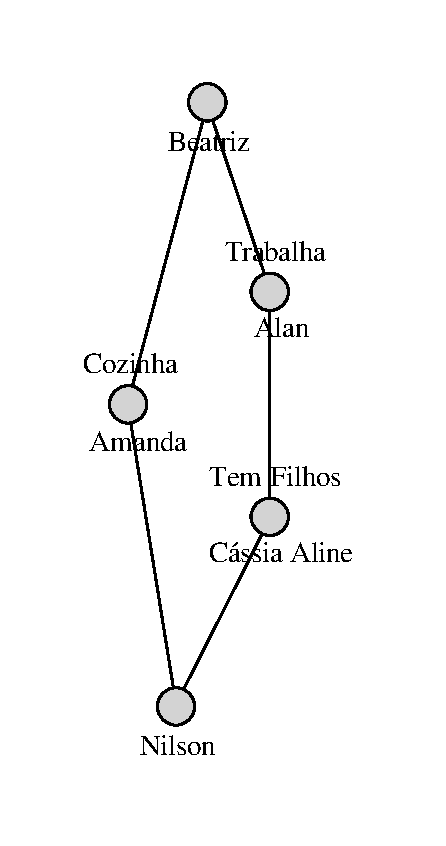
\includegraphics[trim={0pt 2  10 35},clip,height=130pt]{/home/shgo/Dropbox/Doutorado/Palestras/fca/figures/lattice.pdf}
                \caption{Toy example concept lattice.}
            \end{figure}
        \end{column}
    \end{columns}
    $(\{\text{Nilson, Cássia, Aline}\}, \{\text{Tem Filhos, Trabalha, Cozinha}\}) \leq (\{\text{Nilson, Cássia, Aline, Alan}\}, \{\text{Trabalha}\})$
\end{frame}




\begin{frame}[t]{Checklist for FCA}
    \begin{todolist}
        \item[\done] Find a hierarchical order in a set of elements
        \item[\done] Find relationships between two sets
        \item[\done] Find a hierarchical order in a relationship between two sets
    \end{todolist}
\end{frame}

\begin{frame}[c]
    \huge
    How to compute formal concepts?
\end{frame}

\section[Concept Computation]{Formal Concept Computation}
\begin{frame}[t]{Search Space Characterization}
%achar os conceitos pode ser feito computando o conceito para cada combinação de atributos
    From \parencite{Andrews2015}:
    \begin{itemize}
        \item[$\bullet$] Finding all concepts from a context is equivalent to finding all Galois Connections in the form of concepts $(A, B)$, where $B = A^\uparrow, A = B^\downarrow$.
        \item[$\bullet$] In a formal context $(G, M, I)$, for every possible combination of attributes $B \subseteq M$, there is a concept $(B^\downarrow, B^{\downarrow\uparrow})$.
        \item[$\bullet$] We will start by generating all possible combinations of attributes, in a depth-first search.
    \end{itemize}
\end{frame}


\begin{frame}[t]{Search Space Exploration: Naive Approach (\cite{Andrews2015})}
    %mostrar o algoritmo e apontar onde pode ser melhorado
    \begin{algorithm}[H]
        \begin{algorithmic}[1]
            \FOR{$j\leftarrow y$ \TO $n-1$}
            \STATE $K \leftarrow J \cup \{j\}$
            \STATE $A \leftarrow K^\downarrow$
            \STATE $B \leftarrow A^\uparrow$
            \STATE save(A, B)
            \STATE NaiveComputeConceptsOne($K, j + 1$)
            \ENDFOR
        \end{algorithmic}
        \caption{NaiveComputeConceptsOne($J, y$)}
        \label{alg:naive_one}
    \end{algorithm}
    
    \begin{itemize}
        \item[$\bullet$] $J = \emptyset; J = \{0\}; J = \{0, 1\}...$
        \item[$\bullet$] Can we improve this algorithm?
    \end{itemize}
\end{frame}

\begin{frame}[t]{Search Space Exploration: Naive Approach (\cite{Andrews2015})}
%mostrar o algoritmo e apontar onde pode ser melhorado
\begin{algorithm}[H]
\begin{algorithmic}[1]
\FOR{$j\leftarrow y$ \TO $n-1$}
\STATE $K \leftarrow J \cup \{j\}$
\STATE $A \leftarrow K^\downarrow$ \COMMENT{room for improvement}
\STATE $B \leftarrow A^\uparrow$
\STATE save(A, B)
\STATE NaiveComputeConceptsOne($K, j + 1$)
\ENDFOR
\end{algorithmic}
\caption{NaiveComputeConceptsOne($J, y$)}
\label{alg:naive_one_imp}
\end{algorithm}
\end{frame}

\begin{frame}[t]{Search Space Exploration: Naive Approach II (\cite{Andrews2015})}
%mostrar a solução para o problema anterior
\begin{algorithm}[H]
\begin{algorithmic}[1]
\FOR{$j\leftarrow y$ \TO $n-1$}
\STATE $C \leftarrow A \cap \{j\}^\downarrow$
\STATE $B \leftarrow C^\uparrow$
\STATE save(C, B)
\STATE NaiveComputeConceptsTwo($C, j + 1$)
\ENDFOR
\end{algorithmic}
\caption{NaiveComputeConceptsTwo($A, y$)}
\label{alg:naive_two}
\end{algorithm}
\end{frame}

\begin{frame}[t]{Search Space Exploration: First Problem}
    \begin{itemize}
        \item[$\bullet$] The same concept can be computed more than once.
        \item[$\bullet$] The result will be hard to analyze!
    \end{itemize}
    %todo exemplo com bicluster quadrado em várias colunas. Uma combinação das últimas colunas desse bicluster vai gerar o mesmo bicluster.
\end{frame}

\begin{frame}[t]{Search Space Exploration: Compute Once (\cite{Andrews2015})}
    %mostrar a solução para o problema anterior
    \begin{algorithm}[H]
        \begin{algorithmic}[1]
            \FOR{$j\leftarrow y$ \TO $n-1$}
            \STATE $C \leftarrow A \cap \{j\}^\downarrow$
            \STATE $B \leftarrow C^\uparrow$
            \IF{NewConcept($C, B$)}
            \STATE save(C, B)
            \STATE ComputeConceptsOnce($C, j + 1$)
            \ENDIF
            \ENDFOR
        \end{algorithmic}
        \caption{ComputeConceptsOnce($A, y$)}
        \label{alg:naive_once}
    \end{algorithm}
    Still, the concept is computed before checking if it is a new concept!
\end{frame}

\begin{frame}[t]{Combinatorial Problem!}
    \begin{itemize}
        \item[$\bullet$] $\# \text{ possible combs.} = \dbinom{1}{n} + \dbinom{2}{n} + \cdots + \dbinom{n}{n}$
    \end{itemize}
    \begin{figure}
        \centering
        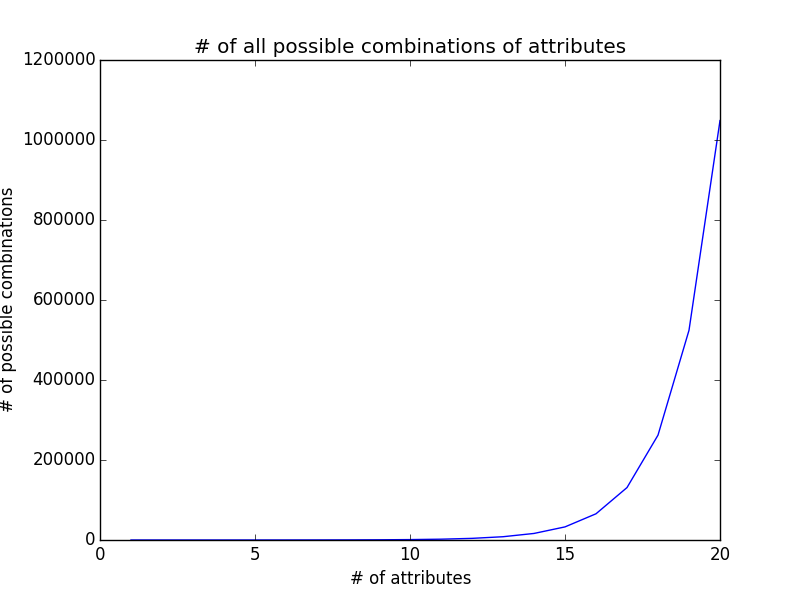
\includegraphics[width=150pt]{all_possible_combinations.png}
        \caption{All possible combinations of attributes, by the number of attributes in a Formal Context.}
    \end{figure}
\end{frame}

\begin{frame}[t]{Canonical Order (\cite{Andrews2015})}
% ordem canonica pode indicar se eu estou computando o mesmo conceito novamente, ou não
    \begin{columns}
        \begin{column}{0.4\textwidth}
            The canonical ordering
                \begin{itemize}
                    \item[$\bullet$] $\{1\} \leq \{2\}$
                    \item[$\bullet$] $\{1\} \leq \{1, 2\}$
                    \item[$\bullet$] $\{1, 2\} \leq \{2\}$
                \end{itemize}
                How can that help?
                \begin{itemize}
                    \item[$\bullet$] $Y_j := \{y \in Y | y < j\}$
                    \item[$\bullet$] $B \cap Y_j = D \cap Y_j$
                \end{itemize}
                %todo exemplo com bicluster quadrado em várias colunas. Uma combinação das últimas colunas desse bicluster vai gerar o mesmo bicluster. Verificar a ordem já dá pra entender que tá repetido.
        \end{column}
        \begin{column}{0.6\textwidth}
            \begin{figure}
                \centering
                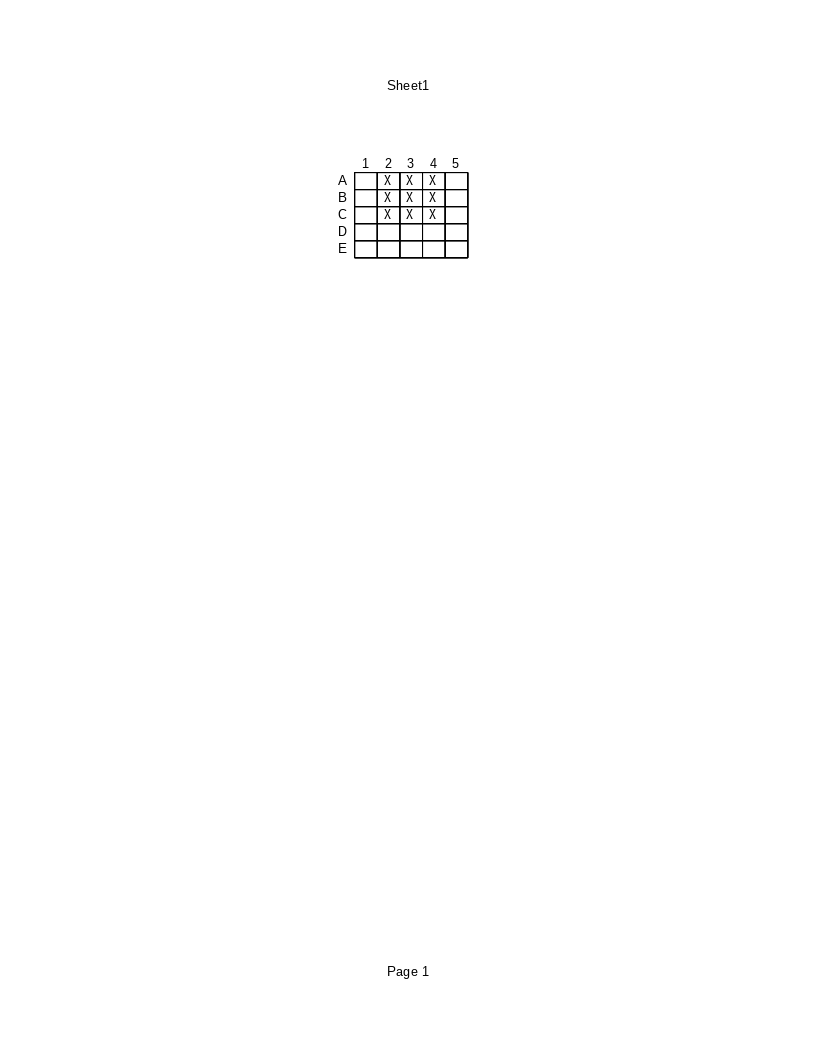
\includegraphics[width=150pt,trim=11cm 28cm 11cm 5cm, clip]{cannonical_example.png}
            \end{figure}
            \begin{itemize}
                \item $\{2\} \implies (\{A, B, C\}, \{2, 3, 4\})$
                \item $\{2, 3\} \implies (\{A, B, C\}, \{2, 3, 4\})$
                \item $\{2, 3, 4\} \implies (\{A, B, C\}, \{2, 3, 4\})$
            \end{itemize}
        \end{column}
    \end{columns}
\end{frame}

\begin{frame}[t]{Search Space Exploration: Close By One (\cite{Andrews2015})}
    %mostra adição da verificação da canonicidade
    \begin{algorithm}[H]
        \begin{algorithmic}[1]
            \STATE save(($A, B$))
            \FOR{$j \leftarrow y$ \TO $n-1$}
                \IF{$j \notin B$}
                    \STATE $C \leftarrow A \cap \{j\}^\downarrow$
                    \STATE $D \leftarrow C^\uparrow$
                    \IF{$B \cap Y_j = D \cap Y_j$}
                        \STATE ComputeConceptsFrom($(C, D)$, $j+1$)
                    \ENDIF
                \ENDIF
            \ENDFOR
        \end{algorithmic}
        \caption{ComputeConcepsFrom(($A, B$), $y$)}
        \label{alg:cbo}
    \end{algorithm}
\end{frame}

\begin{frame}[t]{Search Space Exploration: Close By One (\cite{Andrews2015})}
    %mostra adição da verificação da canonicidade
    \begin{algorithm}[H]
        \begin{algorithmic}[1]
            \STATE save(($A, B$))
            \FOR{$j \leftarrow y$ \TO $n-1$}
                \IF{$j \notin B$}
                    \STATE $C \leftarrow A \cap \{j\}^\downarrow$
                    \STATE $D \leftarrow C^\uparrow$
                    \IF{$B \cap Y_j = D \cap Y_j$}
                        \STATE ComputeConceptsFrom($(C, D)$, $j+1$)
                        \COMMENT{room for improvement}
                    \ENDIF
                \ENDIF
            \ENDFOR
        \end{algorithmic}
        \caption{ComputeConcepsFrom(($A, B$), $y$)}
        \label{alg:cbo_imp}
    \end{algorithm}
\end{frame}

\begin{frame}[t]{Avoiding Computation (\cite{Andrews2015})}
%temos um problema: eu já computei o conceito antes de ver se é novo... E agora?
    How can we avoid computing a concept before checking its canonicity?
    \begin{itemize}
        \item[$\bullet$] Partial closure $A^{\uparrow_j} := \{y \in Y_j | \forall x \in A : xIy\}$
        \item[$\bullet$] Partial closure canonicity test $B \cap Y_j = C^{\uparrow_j}$.
    \end{itemize}
    %todo com o exemplo do bicluster quadrado lá, mostrar que antes mesmo de fechar o bicluster, eu já consigo ver que ele é repetido.
\end{frame}

\begin{frame}[t]{Search Space Exploration: In-Close (\cite{Andrews2015})}
%opa, dá pra ir computando o intent de forma incremental!
    \begin{algorithm}[H]
        \begin{algorithmic}[1]
            \FOR{$j \leftarrow y$ \TO $n-1$}
                \STATE $C \leftarrow A \cap \{j\}^\downarrow$
                \IF{$A = C$}
                    \STATE $B \leftarrow B \cup \{j\}$
                \ELSE
                    \IF{$B = C^{\uparrow_j}$}
                        \STATE $D \leftarrow B \cup \{j\}$
                        \STATE ComputeConceptsFrom(($C, D$), $j + 1$)
                    \ENDIF
                \ENDIF
            \ENDFOR
        \end{algorithmic}
        \caption{ComputeConceptsFrom(($A, B$), $y$)}
        \label{alg:inclose}
    \end{algorithm}
\end{frame}

\begin{frame}[t]{Another Possibilities of Improvement}
%dá pra melhorar ainda mais, só que isso fica pra outro dia. Vejam o Paper!
\begin{itemize}
    \item[$\bullet$] In-Close2: inherited intents (partial closure)
    \item[$\bullet$] FCbO: Failure inheritance + inherited intents (full closure)
    \item[$\bullet$] In-Close3: inherited intents + failure inheritance (partial closure)
\end{itemize}
\end{frame}

\begin{frame}[c]{Comparison By \# of Attributes}
    \begin{figure}
        \centering
        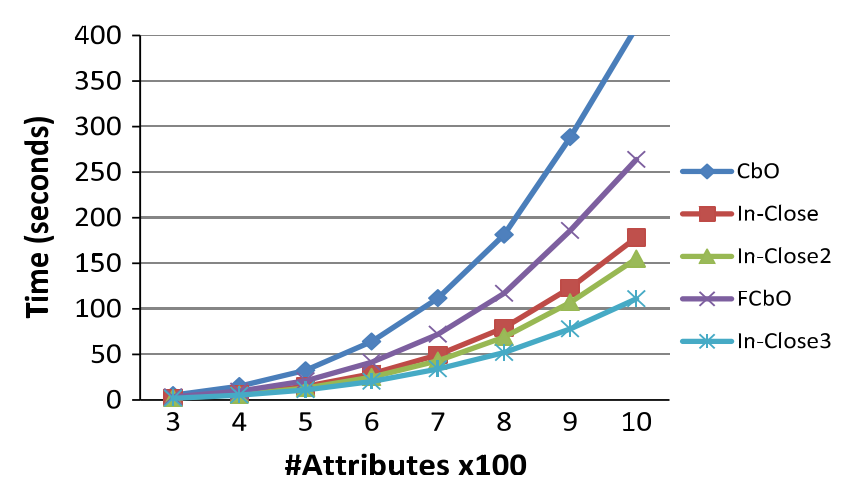
\includegraphics[width=230pt]{andrews_1.png}
        \caption{Comparison of performance with varying number of attributes (300-1000). 5\% density, 5000 objects. \# of concepts approx 1M-22M.
        From \cite{Andrews2015}.}
    \end{figure}
\end{frame}

\begin{frame}[c]{Comparison By Density}
    \begin{figure}
        \centering
        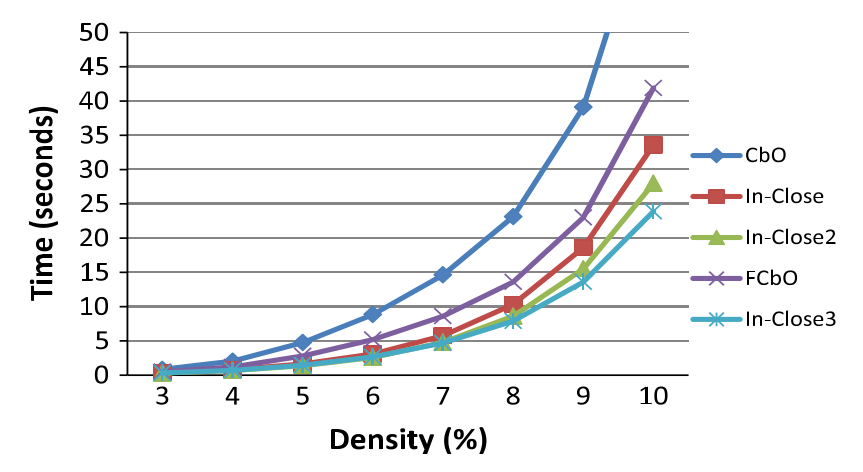
\includegraphics[width=230pt]{andrews_2.png}
        \caption{Comparison of performance with varying context density (3\%-10\%). 200 attributes, 10,000 objects. \# of concepts approx 200m-19M.
        From \cite{Andrews2015}.}
    \end{figure}
\end{frame}

\begin{frame}[c]{Comparison By \# of Objects}
    \begin{figure}
        \centering
        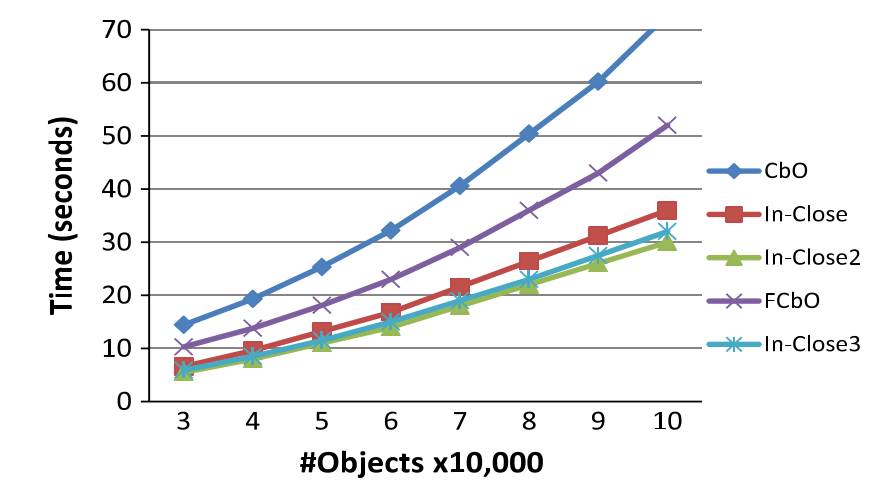
\includegraphics[width=230pt]{andrews_3.png}
        \caption{Comparison of performance with varying number of objects (30m-100m). 5\% density, 200 attributes.
        \# of concepts approx 4M-22M.
        From \cite{Andrews2015}.}
    \end{figure}
\end{frame}

\againframe{toy}

\begin{frame}[t]{An Extension to Graphs}
    %exemplo de animais com relacionamento de x come y. E agora?
    \begin{itemize}
        \item[$\bullet$] How can I include object relationships in my analysis?
    \end{itemize}
    \begin{figure}[h]
        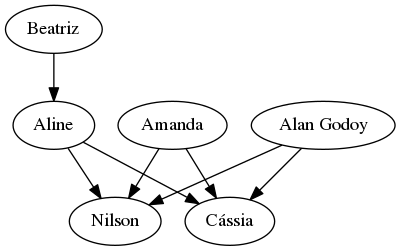
\includegraphics[width=200pt]{/home/shgo/Dropbox/Doutorado/Palestras/fca/figures/chart.png}
        \caption{Toy example object relationships.}
    \end{figure}
\end{frame}

\section[Graph-FCA]{Extending FCA to Graphs}
\begin{frame}[t]{From Dyadic to Graph data}
%os limites da representação diádica, e a codificação de conexões entre objetos que o grafo dá.
    \begin{itemize}
        \item[$\bullet$] We can model object dependence structure by graphs.
        \item[$\bullet$] Several kinds of dependence: (un)directed, hyper-edges, edge-labels...
        \item[$\bullet$] Complex network is a big interdisciplinary research field completely based on graphs.
    \end{itemize}
\end{frame}
\begin{frame}[t]{Can FCA offer good tools for Graph Mining?}
%consigo extender todas aquelas ideias iniciais para grafos? i.e. consigo incluir a relação entre objetos na metáfora de intensão e extensão de um conceito?
    \begin{itemize}
        \item[$\bullet$] Concepts, extension and intension.
        \item[$\bullet$] Generalizing order of graph concepts.
        \item[$\bullet$] New applications for the FCA framework, such as molecule structure investigation, social network analysis, etc.
    \end{itemize}
\end{frame}

\begin{frame}[t]{Checklist for Graph-FCA}
    \begin{todolist}
        \item Graph context
        \item Graph concept extension/intension
        \item Galois connection
        \item Graph concept lattice                
    \end{todolist}
\end{frame}

\begin{frame}[t]{Graph Context}
%vamos tentar. Pra começar, como será representado o nosso contexto formal?
    \begin{definition}[\text{\cite{Ferre2015}}]
        A graph formal context is a triple $K = (O, A, I)$, where $O$ is a set of objects, $A$ is a set of attributes, and $I \subseteq O^* \times A$ is an incidence relation between object tuples and attributes.
        The maximum cardinality of incidences is denoted by $|K|$.
    \end{definition}
    \begin{itemize}
        \item[$\bullet$] Objects are nodes, incidence elements are hyper-edges, and attributes are hyper-edge labels.
    \end{itemize}
\end{frame}

\begin{frame}[t]{Graph Context: Example}
    \begin{figure}[h]
        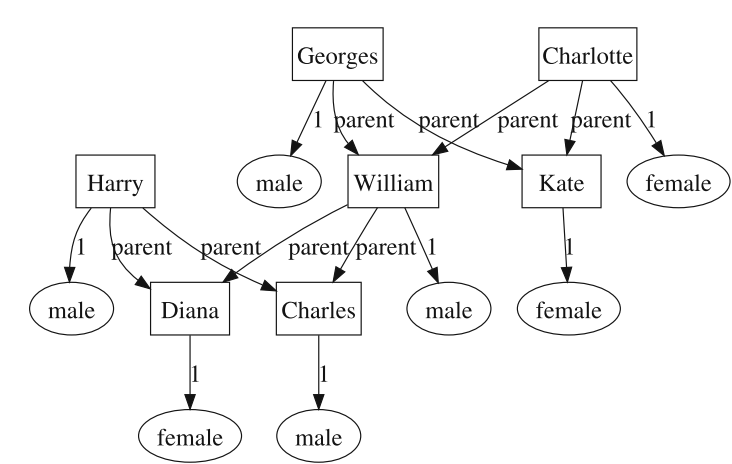
\includegraphics[width=200pt]{/home/shgo/Dropbox/Doutorado/Palestras/fca/figures/knowledge_graph.png}
        \caption{British Royal Family, from \cite{Ferre2015}.}
    \end{figure}
    \begin{itemize}
        \item[$\bullet$] ((Harry, Charles), parent) is a binary incidence relation.
        \item[$\bullet$] ((Diana), female) and ((Charles), male) are unary incidence relations.
    \end{itemize}
\end{frame}

\begin{frame}[t]{Checklist for Graph-FCA}
    \begin{todolist}
        \item[\done] Graph context
        \item Graph concept extension/intension
        \item Galois connection
        \item Graph concept lattice                
    \end{todolist}
\end{frame}

\begin{frame}[t]{Projected Graph Patterns}
%o que eu preciso pra determinar a intenção de um conceito?
    \begin{definition}[\text{\cite{Ferre2016}}]
        A graph pattern $P \subseteq \mathcal{V}^* \times A$ is a set of directed hyperdedges with variables and/or objects as nodes, and attributes as labels.
    \end{definition}
    \begin{definition}[\text{\cite{Ferre2016}}]
        A projected graph pattern (PGP) is a couple $Q = (\bar x, P)$, where $P$ is a graph pattern, and $\bar x \in \mathcal{V}^*$ is called the projection tuple.
        The arity of a PGP is the length of $\bar x$.
        We note $\mathcal{Q}_k$ the set of PGPs having arity $k$.
    \end{definition}
\end{frame}

\begin{frame}[t]{Projected Graph Patterns: Example From \cite{Ferre2016}}
    \begin{columns}
        \begin{column}{0.6\textwidth}
            \begin{figure}[h]
                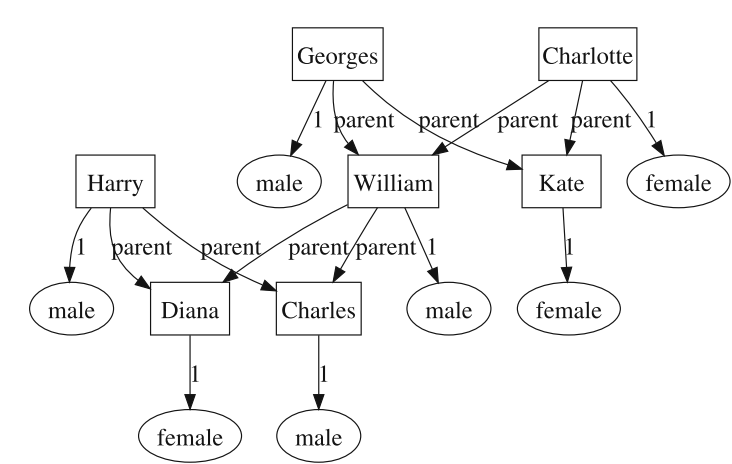
\includegraphics[width=184pt]{/home/shgo/Dropbox/Doutorado/Palestras/fca/figures/knowledge_graph.png}
                \caption{British Royal Family}
            \end{figure}
        \end{column}
        \begin{column}{0.4\textwidth}
            \begin{figure}[h]
                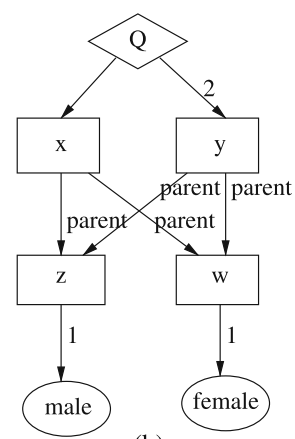
\includegraphics[width=100pt]{/home/shgo/Dropbox/Doutorado/Palestras/fca/figures/pgp_sibiling.png}
                \caption{Sibiling binary relation.}
            \end{figure}
        \end{column}
    \end{columns}
\end{frame}

\begin{frame}[t]{How can we order a set of PGPs?}
    \begin{definition}[\text{\cite{Ferre2016}}]
        A $k$-PGP $Q_1 = (\overline{x_1}, P_1)$ is included in a $k$-PGP $Q_2 = (\overline{x_2}, P_2)$, denoted by $Q_1 \subseteq_q Q_2$, iff there is a mapping $\phi$ from $P_1$-nodes to $P_2$-nodes s.t. $\overline{\phi(x_1)} = \overline{x_2}$, and for every edge $(\overline{y}, a) \in P_1$, $(\overline{\phi(y)}, a) \in P_2$.
    \end{definition}
    \begin{itemize}
        \item[$\bullet$] $\phi$ is a homomorphism from $P_1$ to $P_2$ that preserves the projection tuple and the edges.
        \item[$\bullet$] When $Q_1 \subseteq_q Q_2$ and $Q_2 \subseteq_q Q_1$, they are said equivalent $(Q_1 \equiv_q Q_2)$.
    \end{itemize}
\end{frame}

\begin{frame}[t]{Graph Homomorphism}
    \cite{Brewster}
\end{frame}

\setbeamercolor{background canvas}{bg=}
\includepdf[pages={12-26}]{TutorialBrewster.pdf}

\begin{frame}[t]{How can we order a set of PGPs?}
    \begin{definition}[\text{\cite{Ferre2016}}]
        A $k$-PGP $Q_1 = (\overline{x_1}, P_1)$ is included in a $k$-PGP $Q_2 = (\overline{x_2}, P_2)$, denoted by $Q_1 \subseteq_q Q_2$, iff there is a mapping $\phi$ from $P_1$-nodes to $P_2$-nodes s.t. $\overline{\phi(x_1)} = \overline{x_2}$, and for every edge $(\overline{y}, a) \in P_1$, $(\overline{\phi(y)}, a) \in P_2$.
    \end{definition}
    \begin{itemize}
        \item[$\bullet$] $\phi$ is a homomorphism from $P_1$ to $P_2$ that preserves the projection tuple and the edges.
        \item[$\bullet$] When $Q_1 \subseteq_q Q_2$ and $Q_2 \subseteq_q Q_1$, they are said equivalent $(Q_1 \equiv_q Q_2)$.
    \end{itemize}
\end{frame}

\begin{frame}[t]{Example of PGP inclusion}
    \begin{figure}[h]
        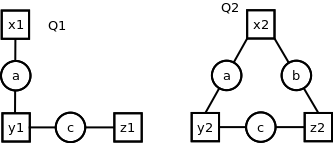
\includegraphics[width=150pt]{/home/shgo/Dropbox/Doutorado/Palestras/fca/figures/PGP_inclusion.png}
        \caption{Example of PGP Inclusion, based on \cite{Ferre2016}.}
    \end{figure}
    \begin{itemize}
        \item[$\bullet$] $Q_1 \subseteq Q_2$
        \item[$\bullet$] $\phi(x_1) = x_2$
        \item[$\bullet$] $\phi(y_1) = y_2$
        \item[$\bullet$] $\phi(z_1) = z_2$
    \end{itemize}
\end{frame}

\begin{frame}[t]{We will also need a PGP intersection $\cap_q$}
    \begin{definition}[\text{\cite{Ferre2016}}]
    Let $\psi$ be an injective mapping from pairs of variables to variables.
    The intersection of two k-PGPs $Q_1 = (\overline{x_1}, P_1)$ and $Q_2 = (\overline{x_2}, P_2)$, denoted by $Q_1 \cap_q Q_2$, is defined as $Q = (\overline{x}, P)$, where $\overline{x} = \overline{\psi(x_1, x_2)}$, and $P = \{(\overline{\psi(y_1, y_2)}, a) | a \in A, (\overline{y_1}, a) \in P_1, (\overline{y_2}, a) \in P_2, |\overline{y_1}| = |\overline{y_2}|\}$.
    \end{definition}
    \begin{itemize}
        \item[$\bullet$] Graph alignment.
        \item[$\bullet$] $\overline{x_1} = \{a_1, b_1, c_1\}, \overline{x_2} = \{a_2, b_2, c_2\}$
        \item[$\bullet$] $\psi(a_1, a_2) = a;$
        \item[$\bullet$] $\psi(a_1, b_2) = b;$
        \item[$\bullet$] $\psi(a_1, c_2) = c;$
    \end{itemize}
\end{frame}

\begin{frame}[t]{Example of PGP intersection $\cap_q$}
    \begin{columns}
        \begin{column}{0.5\textwidth}
            \begin{figure}[h]
                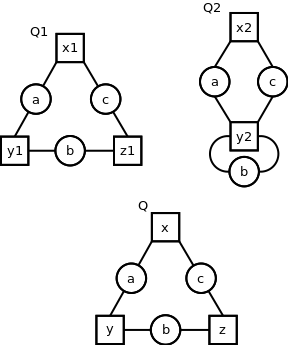
\includegraphics[width=130pt]{/home/shgo/Dropbox/Doutorado/Palestras/fca/figures/PGP_intersection.png}
                \caption{Example of PGP Intersection.}
            \end{figure}
        \end{column}
        \begin{column}{0.5\textwidth}
            \begin{itemize}
                \item[$\bullet$] $\psi(x_1, x_2) = x$
                \item[$\bullet$] $\psi(y_1, y_2) = y$
                \item[$\bullet$] $\psi(z_1, y_2) = z$
            \end{itemize}
        \end{column}
    \end{columns}
\end{frame}

\begin{frame}[t]{Object Relations}
%o que eu preciso pra determinar a extensão de um conceito?
    \begin{definition}[\text{\cite{Ferre2016}}]
        An object relation $\mathcal{R} \subseteq O^k$ is a tuple of objects.
        Its arity is the lenght of the tuple.
        We note $\mathcal{R}_k$ the set of relations with arity $k$.
    \end{definition}
\end{frame}

\begin{frame}[t]{Checklist for Graph-FCA}
    \begin{todolist}
        \item[\done] Graph context
        \item[\done] Graph concept extension/intension
        \item Galois connection
        \item Graph concept lattice                
    \end{todolist}
\end{frame}

\begin{frame}[t]{From Patterns to Relations and Back}
%será que eu consigo relacionar esses dois grupos com uma Galois Connection?
    \begin{definition}[Galois connection, \text{\cite{Ferre2016}}]
        Let $K = (O, A, I)$ be a graph context.
        For every arity $k$, the following pair of mappings between PGPs $Q \in Q_k$ and object relations $R \in \mathcal{R}_k$ forms a Galois connection.
        \begin{center}
            $Q' := \{\overline{o} \in O^k | Q \subseteq_q (\overline{o}, I)\}$
            \hspace{10pt}
            $R' := \cap_q\{(\overline{o}, I) \}_{\overline{o} \in R}$
        \end{center}
    \end{definition}
    \begin{itemize}
        \item[$\bullet$] Very informally: $Q^{'} \approx Q^{\downarrow}$ and $R^{'}\approx R^{\uparrow}$.
    \end{itemize}
\end{frame}

\begin{frame}[t]{Formal Graph Concepts}
%já tenho conceitos então?
    \begin{definition}[\text{\cite{Ferre2016}}]
        A graph concept with arity $k$ is a pair $(R, Q)$, made of an object relation $R \in \mathcal{R}_k$ (the extent) and a PGP $Q \in \mathcal{Q}_k$ (the intent), such that $R = Q'$ and $Q = R'$.
    \end{definition}
    \begin{columns}
        \begin{column}{0.5\textwidth}
            \begin{figure}[h]
                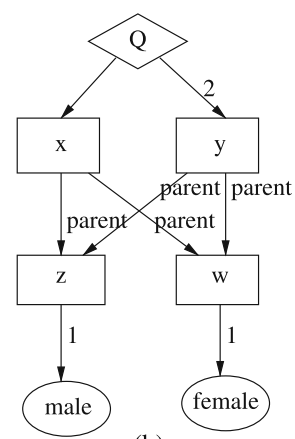
\includegraphics[width=80pt]{/home/shgo/Dropbox/Doutorado/Palestras/fca/figures/pgp_sibiling.png}
                \caption{Sibiling relation PGP, from \cite{Ferre2016}.}
            \end{figure}
        \end{column}
        \begin{column}{0.5\textwidth}
            \begin{itemize}
                \item[$\bullet$] (Harry, William)
                \item[$\bullet$] (Georges, Charlotte)
            \end{itemize}
        \end{column}
    \end{columns}
\end{frame}

\begin{frame}[t]{Checklist for Graph-FCA}
    \begin{todolist}
        \item[\done] Graph context
        \item[\done] Graph concept extension/intension
        \item[\done] Galois connection
        \item Graph concept lattice
    \end{todolist}
\end{frame}

\begin{frame}[t]{Supremum and Infimum}
    \begin{itemize}{}
        \item[$\bullet$] PGP inclusion $\subseteq_q$ is a pre-order over PGPs.
        \item[$\bullet$] PGP Union of a finite collection of PGPs gives us a supremum relative to PGP inclusion.
        \item[$\bullet$] PGP intersection $\cap_q$ gives us an infimum relative to PGP inclusion.
        \item[$\bullet$] Proofs in \cite{Ferre2015}.
    \end{itemize}
\end{frame}

\begin{frame}[t]{Checklist for Graph-FCA}
    \begin{todolist}
        \item[\done] Graph context
        \item[\done] Graph concept extension/intension
        \item[\done] Galois connection
        \item[\done] Graph concept lattice
    \end{todolist}
\end{frame}

\section{Graph-FCA in Practice}
\begin{frame}[t]{Difficulties on Graph-FCA Computation}
    \begin{itemize}
        \item[$\bullet$] Complexity of computing with graphs.
        \item[$\bullet$] Graph Homomorphism.
        \item[$\bullet$] PGP intersection can lead to a bigger graph.
        \item[$\bullet$] How can I find canonical representations of PGPs, like in FCA attributes?
        \item[$\bullet$] In this section, from now on the reference is \cite{Ferre2016}.
    \end{itemize}
\end{frame}

\begin{frame}[t]{Naive Computation}
    \begin{itemize}
        \item[$\bullet$] Generate all combinations of extents (Object Relations).
        \item[$\bullet$] For each one, compute the intent (GPG) using the Galois connection $R' := \cap_q\{(\overline{o}, I)\}_{\overline{o} \in R}$.
    \end{itemize}
\end{frame}

\begin{frame}[t,label=graph_alg]{Efficient Generation of a Concept Basis}
    \begin{algorithm}[H]
        \tiny
        \begin{algorithmic}[1]
            \REQUIRE $K = (O, A, I)$ is a graph context
            \STATE $Concepts \leftarrow \emptyset$
            \STATE $Patterns \leftarrow \{I\}$
            \FORALL{$P \in Patterns$}
                \FORALL{new $P_a \in ConnectedComponents(P \cap_q I)$}
                    \STATE $P_a \leftarrow removeDuplicateNodes(P_a)$
                    \FORALL{new $P_b \in Retracts(P_a)$}
                        \STATE $X \leftarrow P_b.nodes \setminus \bigcup_{R \in Retracts(P_a) | R \subseteq P_b} R.nodes$
                        \IF{$X \neq \emptyset$}
                            \FORALL{$x \in X$}
                                \STATE $Q \leftarrow ((x), P_b); R \leftarrow Q'$
                                \STATE $Concepts \leftarrow \{(R, Q) \in P_b\} \cup Concepts$
                            \ENDFOR
                            \STATE $Patterns \leftarrow \{P_b\} \cup Patterns$
                        \ENDIF
                    \ENDFOR
                \ENDFOR
            \ENDFOR
        \end{algorithmic}
        \caption{Generation of concepts(($A, B$), $y$)}
        \label{alg:gofconcepts}
    \end{algorithm}
\end{frame}

\begin{frame}[t]{\textit{ConnectedComponents($P \cap_q I$)}}
    \begin{block}{How to get all Graph Patterns}
        The algorithm starts by aligning $I$ with itself and using the connected components as Graph Patterns. This alignment is done using the Categorical Product.
    \end{block}
    \begin{definition}
        Let $G$ and $H$ be two graphs.
        The Categorical Product $P = G \times H$ is the graph where $N(P) = N(G) \times N(H)$ and $E(P) = \{[(u, x),(v, y)] : [u, v] \in E(G), [x, y] \in E(H)\}$
    \end{definition}
\end{frame}

\begin{frame}[t]{Graph Categorical Product}
    \cite{Brewster}
\end{frame}

\setbeamercolor{background canvas}{bg=}
\includepdf[pages={128-135}]{TutorialBrewster.pdf}

\againframe{graph_alg}

\begin{frame}[t]{Retracts and Core Graphs}
    \cite{Brewster}
\end{frame}
%core
\setbeamercolor{background canvas}{bg=}
\includepdf[pages={55-58}]{TutorialBrewster.pdf}

%\begin{frame}[c]{Retracts}
%    \begin{figure}[h]
%        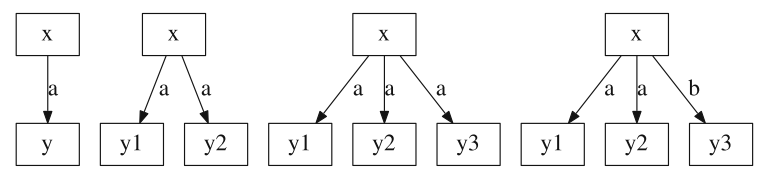
\includegraphics[width=250pt]{/home/shgo/Dropbox/Doutorado/Palestras/fca/figures/retracts.png}
%        \caption{Example of graph retracts.}
%    \end{figure}
%    \begin{block}{Saving Computation}
%        Retracts can be seen as the kernel of a Graph Pattern, and can help saving computation.
%    \end{block}
%\end{frame}

\againframe{graph_alg}

\begin{frame}[t,label=british]{An example}
    \begin{figure}[h]
        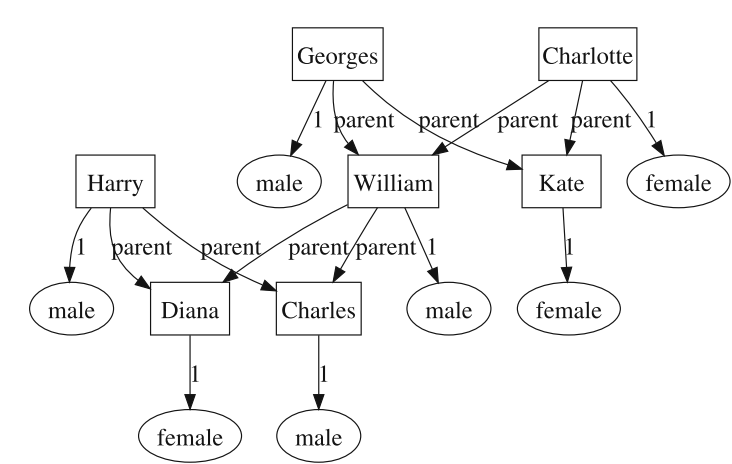
\includegraphics[width=250pt]{/home/shgo/Dropbox/Doutorado/Palestras/fca/figures/knowledge_graph.png}
        \caption{British Royal Family, from \cite{Ferre2016}.}
    \end{figure}
\end{frame}

\begin{frame}[c]{Some Graph Concepts}
    \begin{figure}[h]
        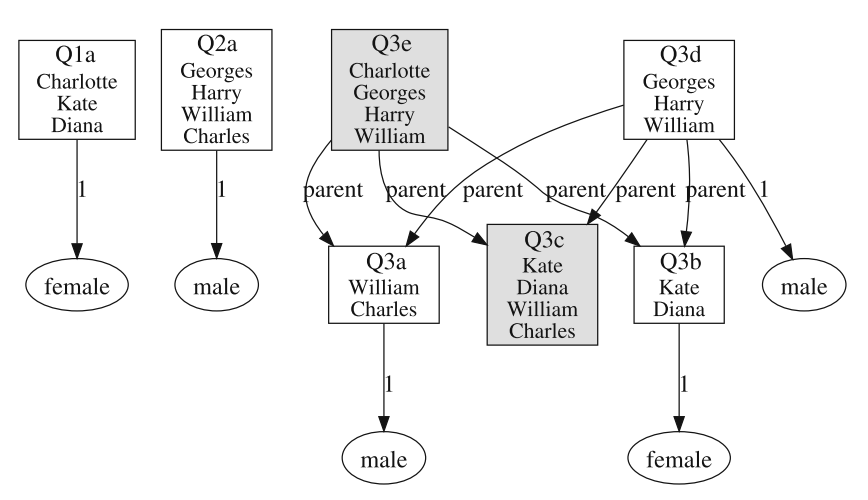
\includegraphics[width=250pt]{/home/shgo/Dropbox/Doutorado/Palestras/fca/figures/graph_concepts.png}
        \caption{British Royal Family}
    \end{figure}
\end{frame}

\begin{frame}[t]{Experiment}
    \begin{itemize}
        \item[$\bullet$] Chocolate apple pie, strawberry-apple pie, mango-coconut pie and gooseberry pie.
        \item[$\bullet$] n-ary relations represent temporal constraints between actions, and entities manipulated by actions.
        For instance, ``put on'': (1) start, (2) end, (3) object, (4) destination.
        \item[$\bullet$] Attributes are action descriptions (e.g., ``cut''), types of ingredients (e.g., ``cream'') or utensils (e.g., ``dish'').
    \end{itemize}
\end{frame}

\begin{frame}[t]{Results}
    \begin{figure}[h]
        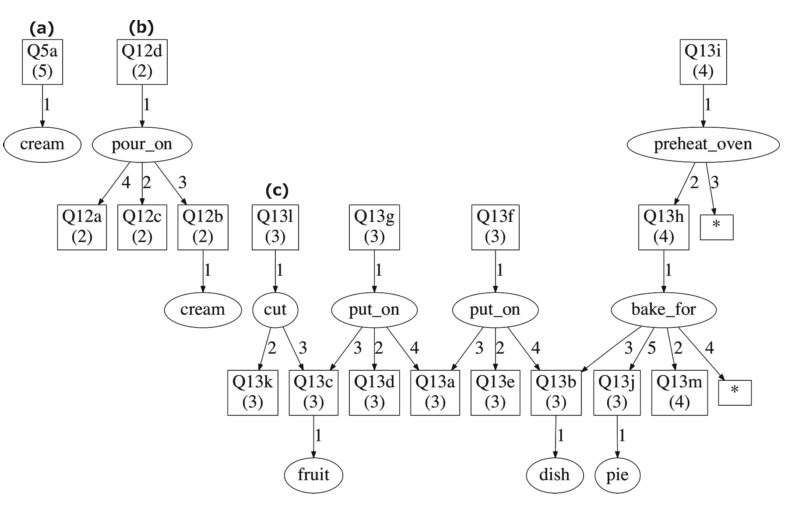
\includegraphics[width=250pt]{/home/shgo/Dropbox/Doutorado/Palestras/fca/figures/recipes.png}
        \caption{Three concepts extracted from the recipes, from \cite{Ferre2016}.}
        \label{fig:recipe_concepts}
    \end{figure}
\end{frame}

\begin{frame}[t]{Results}
    \begin{itemize}
        \item[$\bullet$] Fig. \ref{fig:recipe_concepts}a: ingredients or atomic actions (e.g. ``pour on'').
        \item[$\bullet$] Fig. \ref{fig:recipe_concepts}b: refinements of (a) patterns (e.g. ``pour cream on something'').
        \item[$\bullet$] Fig. \ref{fig:recipe_concepts}c: abstraction of many recipes (e.g. ``cut the fruit in order to put it on something, which is put on a dish, which is baked, after preheating the oven, in order to obtain a pie'').
    \end{itemize}
\end{frame}

\section{Conclusions}
\begin{frame}[t]{Conclusion}
    \begin{itemize}
        \item[$\bullet$] FCA abstraction can be extended in a creative and rigorous way.
        \item[$\bullet$] There are tentatives of generalizing the FCA framework.
        \item[$\bullet$] The experiments showed that Graph Patterns can explain sequential behavior and hidden structure in the network. 
    \end{itemize}
\end{frame}

\begin{frame}[t,allowframebreaks]{References}
    \printbibliography
\end{frame}

\end{document}